% !TEX root = main.tex
\section{Find Alias For Attributes}
\label{sec:fafa}

%For a pair \term{(Sherlock holmes, United Kindom)}, \term{country} is a merely-ok attribute, on the contrary, \term{residence, deathPlace} are better since they are more specific and more seemingly plausible to be an attribute.
%We argue that for each pair of entity, there is a selectional preference for attribute.


%where $f()$ denotes the importance of a concept itself, $g( , )$ denotes the joint ratio of the concepts.
% ENERGY_FUNCTION( f(c1) * f(c2) * g(c1,c2) )


This section is devoted to calculating $s(c_1,c_2)$ of $P((c_{1},c_{2})|(e_{1},e_{2}))$ in Eq.~\ref{eq:target_expand2_jr} and $P((c_{1},c_{2})|a)$ of $P(a|(c_{1},c_{2}))$ in Eq.~\ref{eq:target_expand1}.

According to $P(c_1,c_2|e_1,e_2)$, we can only at concept level indicate the implicit relationship. $P(a|(c_{1},c_{2}))$ retrieves the most probable alias of relation given the concept pair. Thus our objective function solve 2 problems, 1) give out the most probable concept pair of a relation. 2) when multiple relations exist in one concept pair, decide which one is most typical.


\xch{(c1,c2) is only one aspect, any other factor can affect the relation?}


One simple version of the objective function derived from Eq.~\ref{eq:target_expand_all} is equal to Eq.~\ref{eq:simple_obj} when Eq.~\ref{eq:rel_jdp} holds, where we consider $s(c_1,c_2)$ to be how likely the two concepts are going to co-occur.

\begin{equation}
\label{eq:simple_obj}
 \argmax_a \sum_{c_i\in C_1, c_j\in C_2} p((c_{i},c_{j})|a) P(a) P(c_i|e_1) P(c_j|e_2)
\end{equation}

\begin{equation}\label{eq:rel_jdp}
  s(c_1,c_2) = \sum{ P((c_{1},c_{2})|a^*) \times P(a^*)}
\end{equation}

Eq.~\ref{eq:simple_obj} means finding the most probable attribute of $(e_1,e_2)$ by looking at their best concept pair, and find the most probable attribute given the concept pair.



\subsection{Calculating $P((c_{h1},c_{h2})|a)$ }


Given a set of concept pairs (${c_h}_1$,${c_h}_2$), where ${c_h}_1\in C_1$ and ${c_h}_2\in C_2$, we want to find a set of attributes A, where for each $a \in A$:
we can form a (${c_h}_1$,$a$,${c_h}_2$) pair which best describe the relationship between ${c_h}_1$ and ${c_h}_2$.

\begin{example}[Calculating $P(({c_h}_{1},{c_h}_{2}) |a)$]
\label{exa:pggga}
As illustrated in Fig.~\ref{fig:bipartite}, the process of calculating $P(({c_h}_{1},{c_h}_{2}) |a)$ is as follows\term{}
\end{example}


\begin{figure}[!htb]
\centering 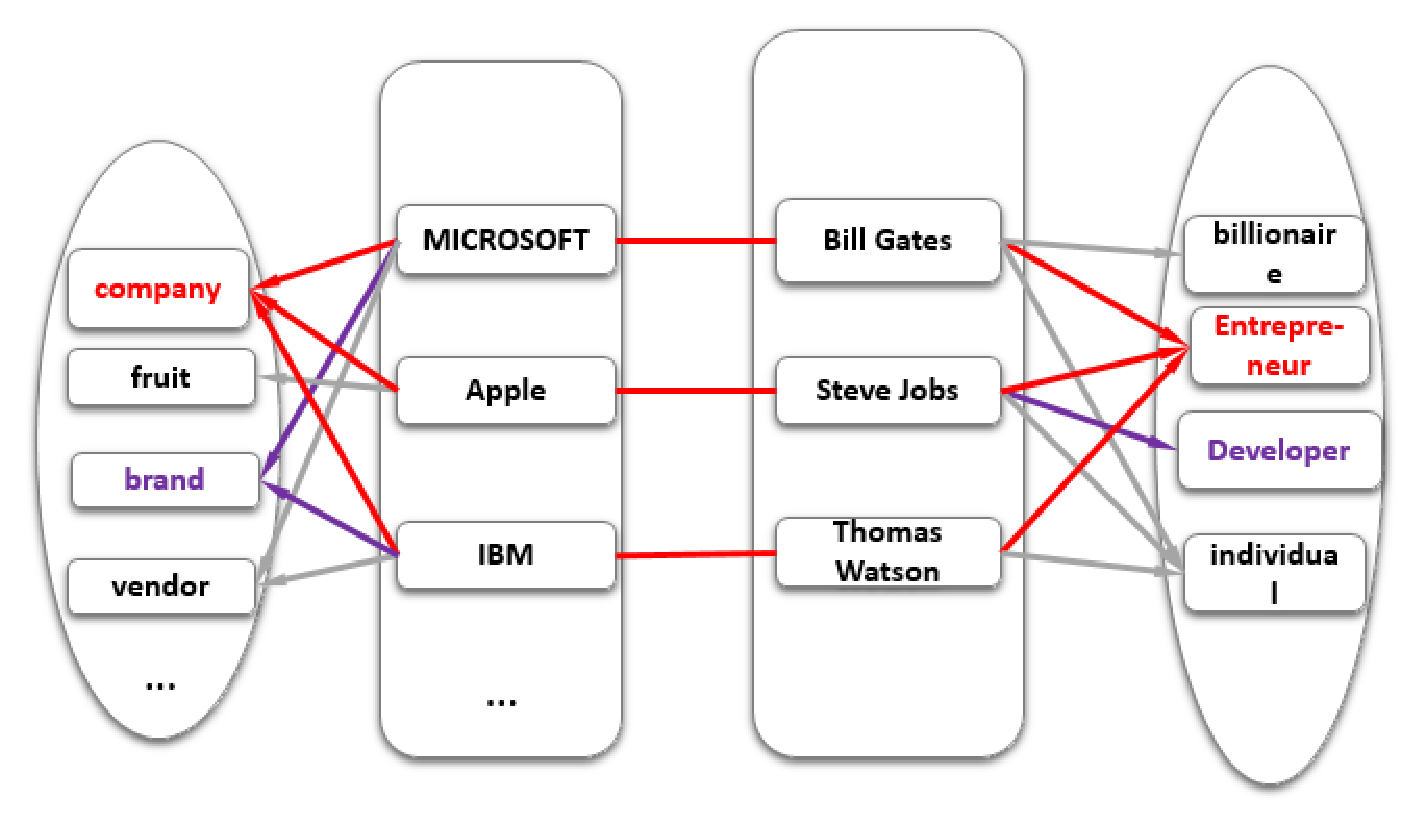
\epsfig{file=resources/ceaec.eps,width=\columnwidth}
\caption{Calculating $P(({c_h}_{1},{c_h}_{2}) |a) $ for \term{FoundedBy}} \label{fig:bipartite}
\end{figure}


For a certain attribute $a_k$, there are many entity pairs of the attribute.
Let $T_k=\{(e_i, a_k, e_j)\}$ be all the triples in the knowledge base with attribute as $a_k$.
\begin{equation}
 P((c_1, c_2) |a_k) = \frac{1}{|T_k|}\sum_{  (e_{i},a_k,e_{j})\in T_k } P(c_1|e_{i})P(c_2|e_{j})
 \end{equation}
Let $C_1$ be all the concepts of $E_L(T_k)$ .... Let $E_L(T_k)$ be all the left entities of attribute $a_k$ in the knowledge base..... We can prove that $\sum_{(c_i,c_j)\in C_1\times C_2} P((c_i, c_j)|a_k)=1$.

\paragraph{Complexity anlaysis}

We first analysis the complexity of calculating $P((c_i, c_j)|a_k)$, manifest in Table.~\ref{tab:complexity}. The original one need to calculate $P((c_i, c_j)|a_k)$ for all $c \in C_1,C_2 $,while most of the concepts are, according to the power law, close to zero, which indicates the rationality of pruning.

% Table generated by Excel2LaTeX from sheet 'Sheet1'
\begin{table}[htbp]
  \centering
  \caption{Complexity Analysis}
    \begin{tabular}{rr}
    \toprule
    method & complexity \\
    \midrule
    original &  $O(|C_1||C_2|)$ \\
    topKpruned & $O(K^2)$ \\
    \bottomrule
    \end{tabular}%
  \label{tab:complexity}%
\end{table}%



To construct the Entity Attribute Graph, we only need topK concepts to form $({c_h}_1,{c_h}_2)$ pair, K trough \xch{case study} is around 5, so we here set K=10.

tuple, later denoted as  $(e_1, a, e_2)$ , where $e_1$ and $e_2$ are also referred to as \term{domain} and \term{range} of the attribute. We can conceptualize $e_1$ and $e_2$ using the method in section~\ref{sec:conceptualization}, and get a set of concept $C_1,C_2$, accompanied with a set of probabilities $P({c_h}_{1}|e_{1i})$, $P({c_h}_{2}|e_2)$,where ${{c_h}_{1} \in C_1},{{c_h}_{2} \in C_2}$.


Thus for any attribute $a$, given a pair of entity $(e_{1i},e_{2j})$, we can define:


\begin{equation} \begin{split} P_{(e_{1i},e_{2j})}(({c_h}_{1},{c_h}_{2}) |a)&=P_{before}({c_h}_1|a) \times P_{after}({c_h}_2|a) \\&=  P({c_h}_{1}|e_{1i}) P(e_{1i}|a) \times P({c_h}_{2}|e_{2j})P(e_{2j}|a) \end{split} \label{eq:giga}\end{equation}


where we use $P_{(e_{1i},e_{2j})}(({c_h}_{1},{c_h}_{2}) |a)$ to denote observing a single pair $(e_{1i},e_{2j})$, how likely is a combination of $({c_h}_{1},a,{c_h}_{2})$ to occur.




Consequently,
\begin{equation} P(({c_h}_{1},{c_h}_{2}) |a)=\sum_{  e_{1i} \in E_1 ,e_{2j} \in E_2} P_{(e_{1i},e_{2j})}(({c_h}_{1},{c_h}_{2}) |a) \label{eq:pg1g2ga}\end{equation}

where $E_1,E_2$ denoting the whole set of domain entity and range entity,The  $P(e_{1i}|a)$ and $P(e_{2j}|a)$ here has only 2 values $1$ and  $0$, depending on whether  $e_1$ occurs before $a$ or $e_2$ occurs after $a$. Apparently, only $(e_{1i}, a, e_{2j})$ occurs will give the equation a non-zero value, therefore, Eq.~\ref{eq:pg1g2ga} is finally equal to Eq.~\ref{eq:gga_fin}.

\begin{equation} \begin{split} P(({c_h}_{1},{c_h}_{2}) |a) &= \sum_{  (e_{1i},a,e_{2j})\in KB } P_{(e_{1i},e_{2j})}(({c_h}_{1},{c_h}_{2}) |a) \\&=  \sum_{  (e_{1i},a,e_{2j})\in KB }P({c_h}_{1}|e_{1i}) \times P({c_h}_{2}|e_{2j})\end{split} \label{eq:gga_fin}\end{equation}

\xch{
The process of calculating \term{} is demonstrated in Example.~\ref{exa:pggga}
}




\subsection{ Calculation of $s(c_1,c_2)$}


$JD(c_1,c_2)$ stands for the joint distribution for $c_1$ and $c_2$, which means how likely $c_2$ is going to appear as an attribute's concept of $c_1$.

\begin{definition}[Definition of $JD(c_1,c_2)$]

  $$ JD(c_1,c_2) = \frac{1}{Z_\theta}\times e^{- \frac{1}{f(c_1)\times f(c_2)\times g(c_1,c_2))}},$$
  where $$f(c_i)=\sum{ P(c_i|e^*) },(i=1,2)$$
  denotes the typicality of a concept itself, $$g({c_h}_1 ,{c_h}_2 )=\sum P({c_h}_{1}|e_{1i}^*) \times P({c_h}_{2}|e_{2j}^*)$$
  denotes the joint ratio of the concepts.


\end{definition}




\xch{ ==============problem here!!! the numerator and the denominator multiplies and get 1, is the relationship here correct??==========}

We first specify the relationship between $P((c_{1},c_{2})|a^*) $ and $JD(c_1,c_2)$. Actually, they have the following relationship:
\xch{===========================}



To Construct the Entity Attribute Graph, we calculate $P(({c_h}_{1},{c_h}_{2}) |a)$ for each attribute.




Note that we only consider the attributes whose range is an entity, and ignore those numerical values or date-and-time values such as $( Mona Lisa, Year, 1503)$.





For each $({c_h}_{1},a,{c_h}_{2})$ tuple, we can calculate $P(({c_h}_{1},{c_h}_{2}) |a)$ for each







%\subsubsection{Voting}


%\subsection{For multiple hops}
%
%\subsubsection{Entity Attribute Graph Construction}
%
%
%\begin{figure}[!htb]
%\centering 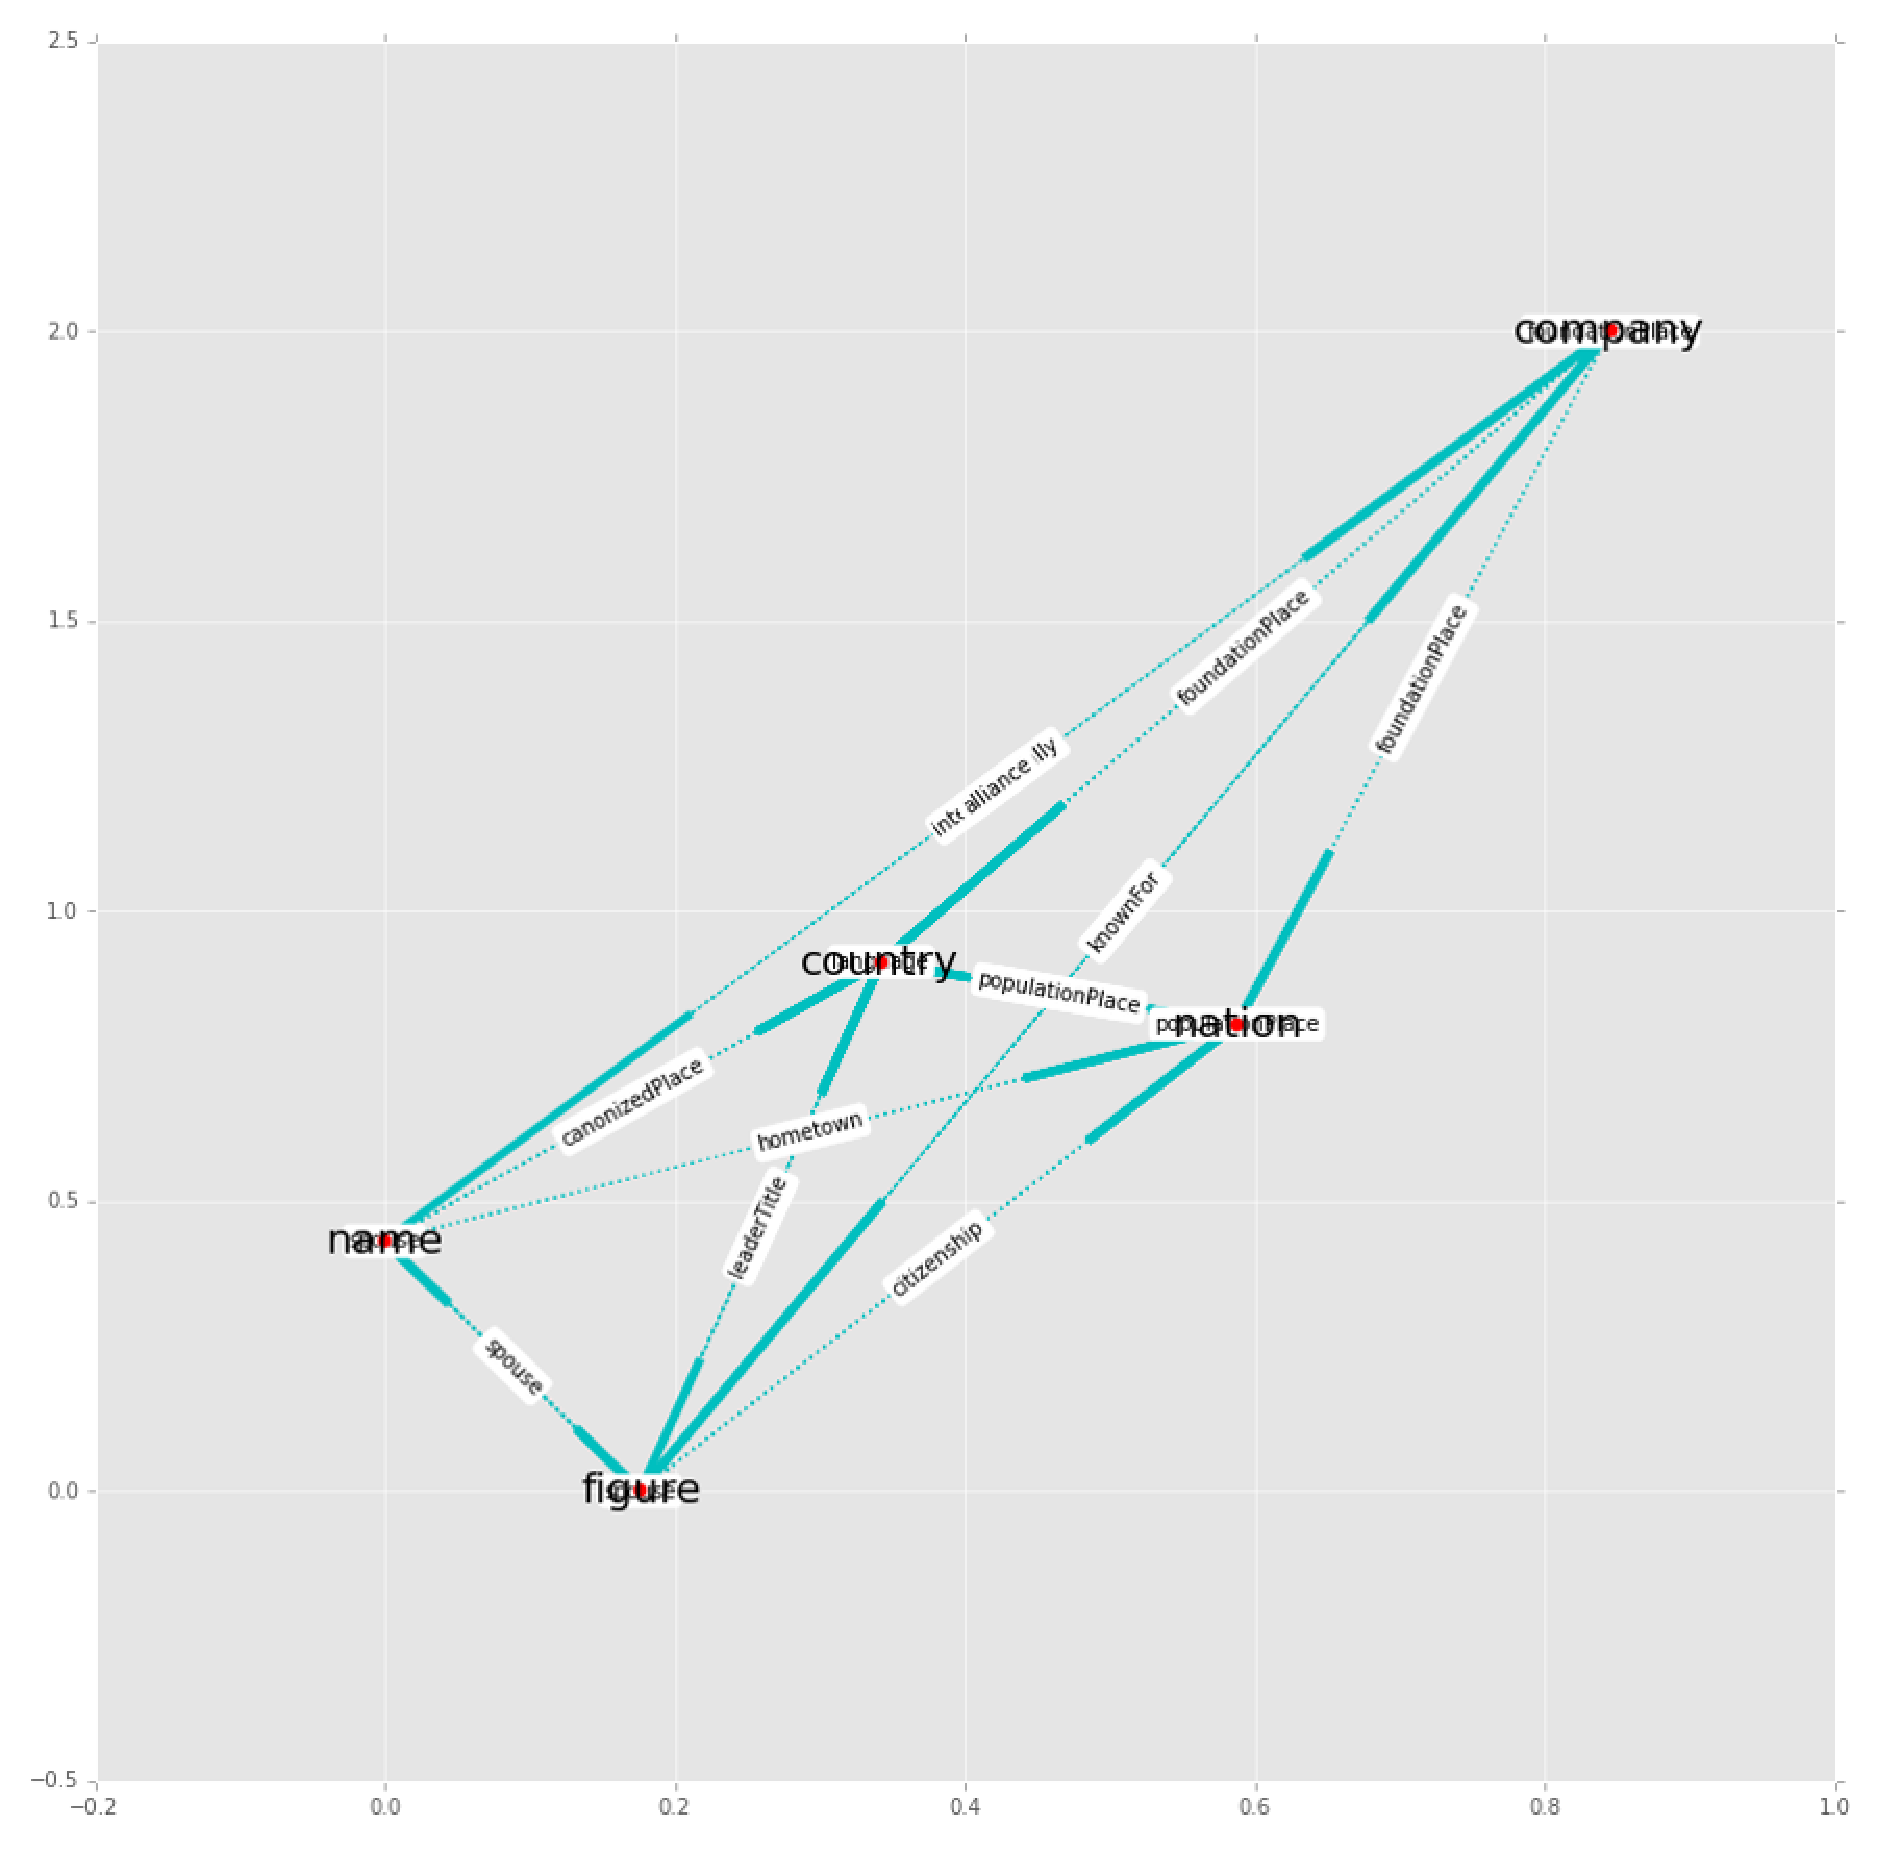
\epsfig{file=resources/eag.eps,width=2.5in}
%\caption{Subgraph of Entity Attribute Graph } \label{fig:eag}
%\end{figure}
%
%So far, we have tackled with the relations and generated the edges in the relationship graph.
%This problem is similar to {\bf hierarchy ranking problems in a directed graph}~\cite{gupte2011finding}. Originally, it was a minimum feedback arc set problem on a weighted network which is a classic NP-hard problem~\cite{dinur2005hardness}. A few approaches~\cite{tatti2014faster} have been proposed on unweighted directed graphs, for weighted graphs, the extended agony[hierarchies in directed network(unpublished kdd15)] algorithm can be ultilized to generate hierarchy results \xch{in this approach the K (number of hierarchies) is fixed, maybe we can make it adaptive to data here? }
%
%
%
%In this section, we first formulate the problem of finding semantic link into a maximum flow problem on the concept network with multiple-sources and multiple-sinks, and then, we cut out the subgraph and perform {\bf improved agony} to derive the concept of the middle entities. Last we use co-occurrence to verify the validness of the relation.
%
%%We argue that co-occurrences between entities can only be applied to entity relation explanation when they are conceptually correct[]. Following this intuition, we further formalize our problem into
%
%
%\subsubsection{Improved agony}
%
%



%\subsection{Find the best alias}
%
%We then Use an $\argmax$ model \xch{use KL divergence? to minimize $D_{KL}{}$} to solve the problem.
%
%Given $(e_1,e_2)$, our goal is to find the best attribute for it. We denote it as:
%$$\argmax P((e_1,e_2)|a) $$
%where
%$$P((e_1,e_2)|a)= $$

